\chapter{Avaliação}
\label{chapter:evaluation}

Conforme apresentado no \autoref{chapter:proposal}, a etapa de medição do \textit{pipeline} produz uma matriz de similaridade entre os testes decompostos. Essa matriz constitui a base para identificar pares de testes candidatos à refatoração por meio da configuração implícita e, posteriormente, para o agrupamento global da suíte. Antes que o agrupamento e a refatoração automática possam ser avaliados de ponta a ponta no Róża, é necessário verificar se as métricas de similaridade recuperam, com precisão aceitável, os pares de testes que de fato podem compartilhar código de configuração de acessórios.

Este capítulo apresenta o experimento conduzido para comparar as cinco métricas disponíveis no Róża (JPlag, Simian, Deckard, LCS e LCCSS) quanto à sua capacidade de identificar pares de testes adequados à refatoração por configuração implícita. O experimento foi originalmente relatado em \citeonline{silva:etal:2020} e reúne, nesta versão do trabalho, a metodologia, os resultados e as ameaças à validade alinhados à terminologia e à arquitetura em \textit{pipeline} adotadas aqui. A avaliação da redução de duplicação e do esforço de refatoração após o agrupamento e a reconstrução das classes de teste permanece dependente da implementação das etapas subsequentes do \textit{pipeline}; o experimento aqui descrito constitui, portanto, a avaliação empírica da etapa de medição, inclusive da métrica LCCSS.

\section{Objetivo e desenho do experimento}

O objetivo do experimento consiste em comparar métricas de similaridade quanto à sua eficácia em recuperar pares de testes classificados manualmente como candidatos à refatoração por configuração implícita. Para isso, adota-se a perspectiva de recuperação da informação \cite{baezayates:etal:1999}: para cada teste da suíte, a métrica em avaliação produz uma ordenação dos demais testes por grau de similaridade decrescente; essa ordenação é confrontada com um conjunto de referência de pares compatíveis, elaborado pelos autores por meio de classificação manual.

O experimento divide-se em cinco fases, executadas em sequência: (1) seleção da fonte de dados; (2) classificação manual e construção da matriz de controle; (3) geração de variantes de configuração para cada métrica; (4) execução de cada variante e obtenção das matrizes de similaridade; e (5) coleta dos resultados por meio de curvas médias de precisão e recaptação (\textit{precision/recall}). As fontes, os \textit{scripts} e as instruções de replicação encontram-se no repositório público do Róża\footnote{\url{https://github.com/lucasPereira/roza/tree/master/experiment-results}}\footnote{\url{https://github.com/lucasPereira/roza/tree/master/src/expt}}.

A \autoref{figure:experiment-phases} sintetiza esse fluxo e explicita os artefatos transferidos entre as fases. Na primeira fase, a suíte de testes de aceitação é filtrada segundo critérios de compatibilidade com o processamento do Róża, resultando no conjunto de 46 testes que alimenta as etapas seguintes.

Na segunda fase, os autores classificam manualmente cada um dos 1035 pares distintos formados por esses testes e constroem a matriz de controle binária, na qual cada célula indica se a refatoração por configuração implícita seria adequada (1) ou inadequada (0); a partir dessa matriz, derivam-se os conjuntos de testes compatíveis que servirão de referência na avaliação.

Na terceira fase, após a construção da matriz de controle, definem-se as variantes de configuração de cada métrica. JPlag, Simian e Deckard admitem parâmetros de sensibilidade que alteram a detecção de trechos semelhantes; a LCS e a LCCSS não exigem ajuste e constituem variantes únicas. O diagrama resume o cardinal dessas variantes: 51 para JPlag, 14 para Simian, 476 para Deckard, 1 para LCS e 1 para LCCSS.

Na quarta fase, cada variante é aplicada ao conjunto de testes selecionado, produzindo uma matriz de similaridade com graus numéricos entre todos os pares de testes. A partir de cada matriz, gera-se, para cada teste, uma ordenação dos demais testes por grau de similaridade decrescente.

Na quinta fase, confrontam-se as ordenações produzidas por cada variante com os conjuntos de testes compatíveis da matriz de controle e calculam-se curvas médias de precisão e recaptação; para cada métrica, seleciona-se a variante de melhor desempenho para a análise comparativa final.

\begin{figure}[htb]
	\centering
	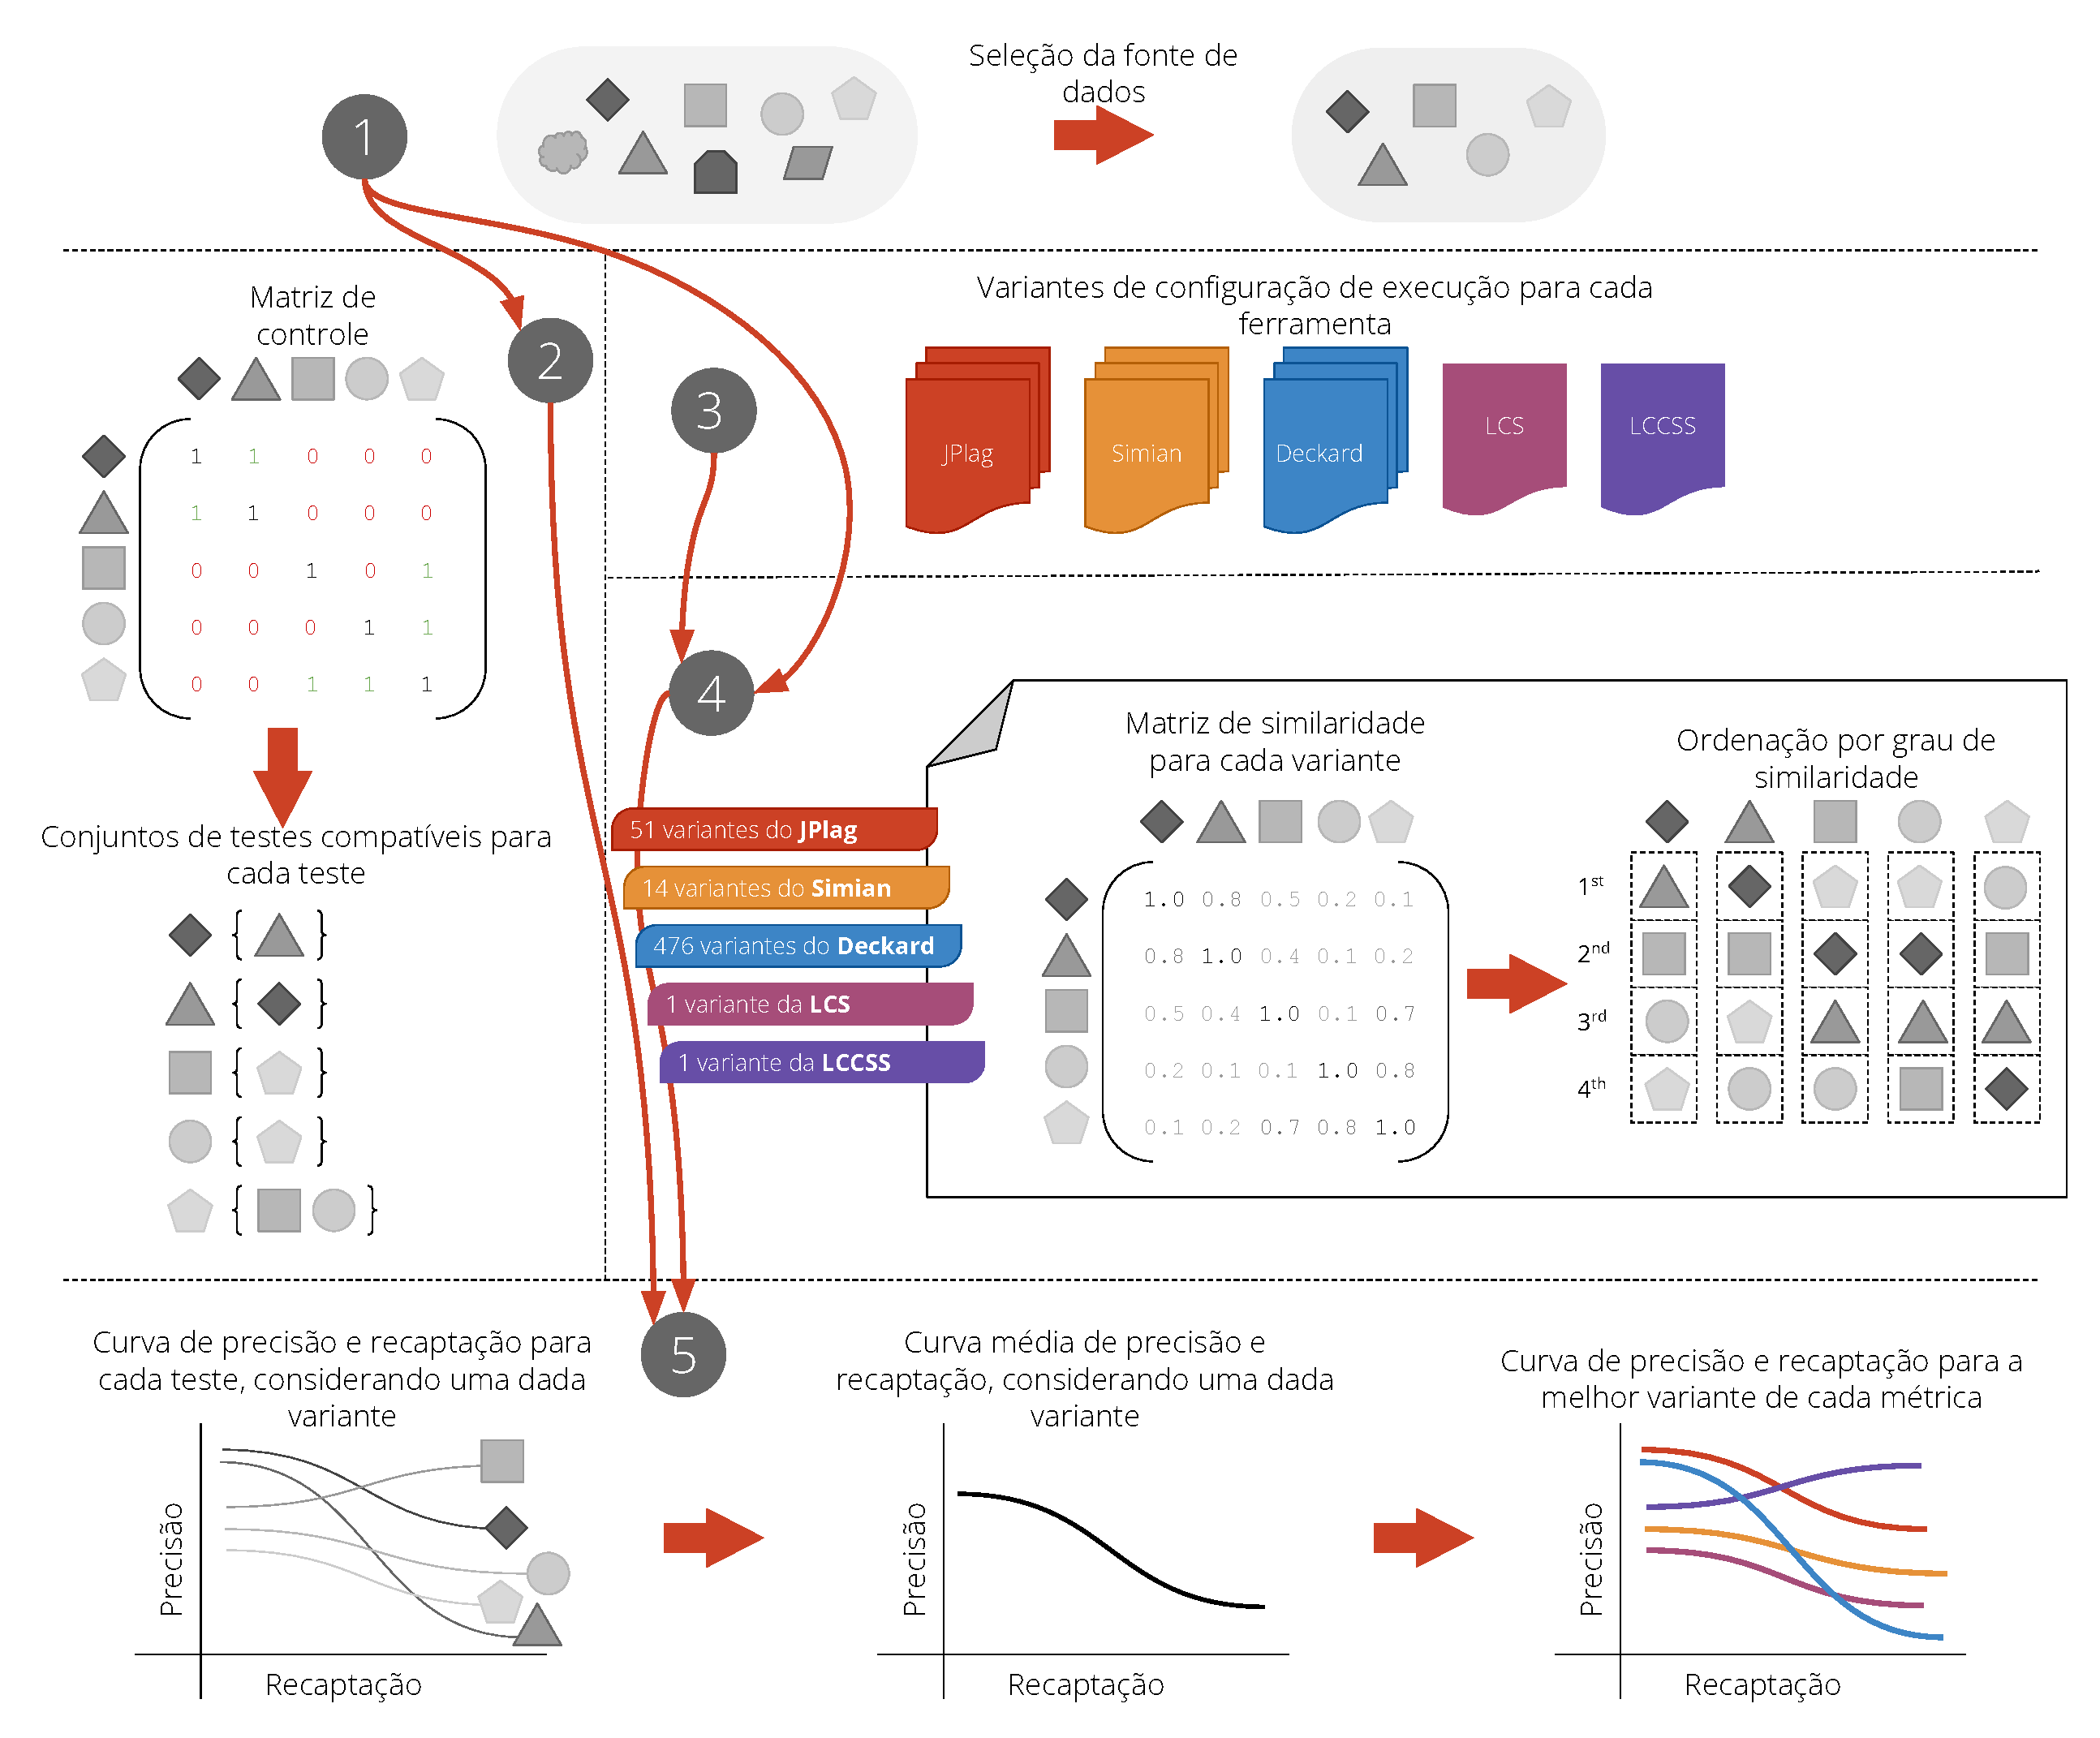
\includegraphics[width=0.75\textwidth]{figures/experiment-phases.pdf}
	\caption{Fases do experimento de avaliação das métricas de similaridade}
	\label{figure:experiment-phases}
	\fonte{Elaborado pelo autor.}
\end{figure}

\section{Fonte de dados}

A fonte de dados consiste em 46 testes de aceitação em nível de sistema, escritos em Java com JUnit e extraídos de um sistema para avaliação de produções de livros desenvolvido para a Coordenação de Aperfeiçoamento de Pessoal de Nível Superior (CAPES). Esse sistema é um \textit{fork} do projeto de código aberto \textit{Open Monograph Press} (OMP)\footnote{\url{https://github.com/pkp/omp}}. Selecionaram-se os testes do \textit{fork} por serem compatíveis com o processamento do Róża, enquanto os testes originais do OMP, escritos em PHP, foram excluídos. Os 46 testes utilizam Selenium\footnote{\url{https://selenium.dev/}} para controlar o navegador e estão distribuídos em seis classes de teste, com média de 209 linhas de código por classe.

\section{Matriz de controle}

Na segunda fase, os 1035 pares distintos formados pelos 46 testes foram classificados manualmente. Para cada par, respondeu-se à seguinte pergunta: é adequado colocar os dois testes na mesma classe de teste a fim de reusar código de configuração de acessórios por meio da configuração implícita? Por adequado, entende-se que o reuso obtido por refatoração manual seria relevante o suficiente para compensar o esforço de reorganização.

Dessa análise resultaram 219 pares classificados como adequados à refatoração por configuração implícita e 816 pares classificados como inadequados. Para reduzir viés e erro humano, a classificação foi realizada duas vezes e os casos conflitantes foram reanalisados. A partir da matriz binária de controle, gerou-se, para cada teste, o conjunto de testes compatíveis (i.e., os demais testes com os quais poderia compartilhar um método de configuração implícita). Esses conjuntos alimentam a quinta fase do experimento.

\section{Variantes de configuração}

JPlag, Simian e Deckard admitem parâmetros que alteram a sensibilidade da detecção de trechos semelhantes; a LCS e a LCCSS não exigem configuração. Para assegurar comparação justa entre as métricas parametrizáveis, gerou-se o produto cartesiano dos valores candidatos de cada parâmetro, conforme a Tabela~\ref{table:metric-settings}. A variante com melhor desempenho médio de precisão nos onze níveis padrão de recaptação foi selecionada para representar cada métrica na análise final.

\begin{table}[htb]
	\centering
	\caption{Parâmetros e valores utilizados na geração de variantes de configuração}
	\label{table:metric-settings}
	\small
	\begin{tabular}{llcc}
		\toprule
		Métrica & Parâmetro & Valores & Variantes \\
		\midrule
		JPlag & sensibilidade (\texttt{-t}) & 1 a 50 & 51 \\
		\midrule
		Simian & limiar de linhas (\texttt{-threshold}) & 2 a 15 & 14 \\
		\midrule
		\multirow{3}{*}{Deckard} & \texttt{MIN\_TOKENS} & 1 a 15 & \multirow{3}{*}{476} \\
		                         & \texttt{STRIDE} & 0 a 15 e \texttt{inf} & \\
		                         & \texttt{SIMILARITY} & 0,9 e 1,0 & \\
		\midrule
		LCS & nenhum & --- & 1 \\
		LCCSS & nenhum & --- & 1 \\
		\bottomrule
	\end{tabular}
\end{table}

Os intervalos de valores tomaram como referência os padrões de cada ferramenta e os valores empregados por \citeonline{ragkhitwetsagul:etal:2018} em experimentos com detectores de clones.

\section{Execução}

Na quarta fase, cada variante de configuração foi aplicada aos 46 testes por meio do Róża, produzindo uma matriz de similaridade simétrica ou assimétrica conforme a métrica. A partir de cada matriz, obteve-se, para cada teste, o grau de similaridade de cada candidato; ordenados do maior para o menor, esses valores constituem a saída comparada com os conjuntos de testes compatíveis definidos na matriz de controle.

\section{Métricas de avaliação e resultados}

Na quinta fase, confrontam-se as ordenações produzidas por cada variante com o gabarito definido na segunda fase. O procedimento pode ser lido em três etapas sucessivas: primeiro, para cada um dos 46 testes de referência, gera-se uma curva de precisão e recaptação a partir da ordenação da variante em relação a esse teste; em seguida, tira-se a média dessas 46 curvas, obtendo a curva da variante; por fim, escolhe-se a melhor variante dentro de cada métrica.

Para cada teste de referência $T$, o gabarito é um conjunto $C(T)$ de testes compatíveis. A variante em avaliação, por sua vez, atribui um grau de similaridade a cada candidato e produz uma ordenação dos demais testes, do maior para o menor grau. A avaliação verifica se os candidatos que a métrica coloca no topo dessa ordenação coincidem com $C(T)$.

A geração das curvas percorre a ordenação do candidato mais similar ao menos similar. Cada nível padronizado de recaptação (0\%, 10\%, \ldots, 100\%) corresponde a uma fração dos compatíveis que deve ser recuperada: no nível de 10\%, por exemplo, exige-se recuperar 10\% dos elementos de $C(T)$; no de 50\%, metade deles. Calcula-se, para cada nível, quantos elementos de $C(T)$ essa fração representa; a ordenação é percorrida candidato a candidato, do topo em diante, até recuperar essa quantidade. Com o prefixo definido, a precisão é a proporção de candidatos recuperados que o gabarito classifica como compatíveis. Isso produz, para cada teste, onze pares de recaptação e precisão.

A agregação seguinte condensa as 46 curvas individuais em uma curva por variante. Para cada nível de recaptação, calcula-se a média aritmética das 46 precisões observadas naquele nível. Em outras palavras, fixa-se a recaptação (por exemplo, 50\%) e tira-se a média das precisões que os 46 testes atingiram nesse nível; repete-se para os onze níveis.

O exemplo a seguir ilustra o cálculo para o teste \texttt{importarProducoesComSucesso} com a variante JPlag de sensibilidade 23. Para esse teste, o gabarito contém oito testes compatíveis, todos da mesma funcionalidade de importação de produções. Já a ordenação produzida pela métrica coloca, no topo, testes de outras funcionalidades com grau elevado (e.g., \texttt{importar\-Avaliadores\-Coordenador\-ComSucesso}); por isso, sua precisão é penalizada. Por exemplo, considerando o nível de recaptação de 20\%, é necessário recuperar um teste compatível ($\lfloor 0{,}2 \times 8 \rfloor = 1$); o menor prefixo que atinge essa meta na variante tem 16 candidatos, o que significa uma precisão de $1/16 = 0{,}0625$, ou seja, o primeiro candidato compatível encontrado estava na 16\textsuperscript{a} posição. Na recaptação de 50\%, recuperam-se quatro compatíveis em um prefixo de 19 candidatos (precisão $\approx 0{,}2105$); em 100\%, os oito compatíveis exigem um prefixo de 33 candidatos (precisão $\approx 0{,}2424$). Os onze pontos acima formam a curva de precisão e recaptação. Na agregação, em cada nível de recaptação, calcula-se a média aritmética das precisões dos 46 testes de referência, gerando a curva média de precisão e recaptação.

A seleção da melhor variante ocorre dentro de cada métrica. Para cada variante, calcula-se a média aritmética das onze precisões da curva agregada; permanece a configuração de maior média. A LCS e a LCCSS não possuem parâmetros e constituem variantes únicas. Quando duas configurações da mesma métrica produzem a mesma curva agregada (e.g., JPlag de sensibilidade 23 a 32), qualquer uma delas representa o desempenho da métrica; adota-se a de menor sensibilidade entre as empatadas.

Esse procedimento segue a perspectiva de recuperação da informação \cite{baezayates:etal:1999}. Diz-se que um candidato foi recuperado quando seu grau de similaridade em relação ao teste de referência se encontra entre os mais elevados; a precisão é a fração de recuperados que a matriz de controle classifica como compatíveis, e a recaptação é a fração dos compatíveis desse teste que foram recuperados em cada um dos onze níveis padronizados.

A Tabela~\ref{table:best-configurations} apresenta a melhor variante de configuração selecionada para JPlag, Simian e Deckard. A LCS e a LCCSS não possuem parâmetros e, por isso, não aparecem na tabela.

\begin{table}[htb]
	\centering
	\caption{Melhores variantes de configuração por métrica}
	\label{table:best-configurations}
	\small
	\begin{tabular}{llc}
		\toprule
		Métrica & Parâmetro & Valor \\
		\midrule
		JPlag & sensibilidade (\texttt{-t}) & 23 \\
		\midrule
		Simian & limiar de linhas (\texttt{-threshold}) & 8 \\
		\midrule
		\multirow{3}{*}{Deckard} & \texttt{MIN\_TOKENS} & 9 \\
		                         & \texttt{STRIDE} & 11 \\
		                         & \texttt{SIMILARITY} & 1,0 \\
		\bottomrule
	\end{tabular}
\end{table}

A \autoref{figure:precision-recall-curves} apresenta uma linha para a melhor variante de cada métrica. O eixo horizontal percorre onze níveis padrão de recaptação, de 0\% a 100\% em incrementos de 10\%, e o eixo vertical registra a precisão média correspondente, considerando todos os testes da suíte.

\begin{figure}[htb]
	\centering
	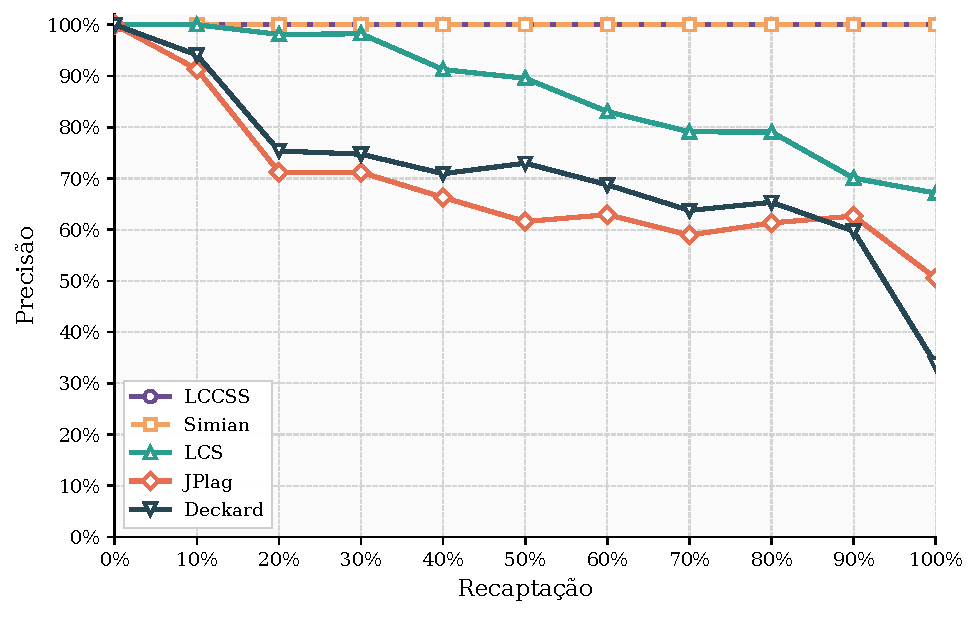
\includegraphics[width=\textwidth]{figures/precision-recall-curves.pdf}
	\caption{Curvas médias de precisão e recaptação para a melhor variante de cada métrica}
	\label{figure:precision-recall-curves}
	\fonte{Elaborado pelo autor.}
\end{figure}

Como se observa na \autoref{figure:precision-recall-curves}, todas as métricas alcançaram precisão superior a 0,9 no nível de recaptação de 10\%. Entretanto, JPlag, Deckard e LCS apresentaram queda de precisão à medida que a recaptação aumenta, o que indica crescimento de falsos positivos quando se exige recuperar proporções maiores dos pares compatíveis. Em contraste, LCCSS e Simian mantiveram precisão 1,0 em todos os onze níveis de recaptação: todos os pares classificados como compatíveis foram recuperados sem falsos positivos nas ordenações produzidas por essas duas métricas. Por apresentarem os mesmos valores, as curvas dessas duas métricas ficam sobrepostas no gráfico.

A Tabela~\ref{table:average-similarity-degrees} resume os graus médios de similaridade atribuídos por cada métrica na melhor variante. Simian e LCCSS apresentam as menores médias e os maiores desvios padrão, padrão coerente com a matriz de controle, na qual apenas 219 dos 1035 pares (cerca de 21\%) foram considerados compatíveis: a maior parte dos pares recebe grau baixo e uma minoria recebe graus mais elevados. As demais métricas distribuíram graus de forma mais uniforme, o que dificulta separar pares compatíveis de incompatíveis e explica a queda de precisão observada nas curvas.

\begin{table}[htb]
	\centering
	\caption{Graus médios de similaridade na melhor variante de cada métrica}
	\label{table:average-similarity-degrees}
	\small
	\begin{tabular}{lcccc}
		\hline
		Métrica & Média & Desvio padrão & Mínimo & Máximo \\
		\hline
		JPlag & 0,73 & 0,18 & 0,00 & 1,00 \\
		Simian & 0,13 & 0,25 & 0,00 & 0,90 \\
		Deckard & 0,33 & 0,13 & 0,19 & 1,00 \\
		LCS & 0,66 & 0,13 & 0,38 & 0,98 \\
		LCCSS & 0,23 & 0,25 & 0,05 & 0,98 \\
		\hline
	\end{tabular}
\end{table}

\section{Discussão dos resultados}

A análise qualitativa dos graus atribuídos por LCS, JPlag e Deckard revela um padrão comum de falsos positivos: trechos comuns situados fora do prefixo inicial das configurações de acessórios elevam o grau de similaridade mesmo quando a configuração implícita não pode extrair esse código com segurança, conforme ilustrado na \autoref{figure:lccss-lcs-comparison}. A LCS, em particular, atribui graus elevados quando o final das configurações coincide, embora o início diverja. JPlag e Deckard, por sua vez, podem atribuir graus baixos a pares cujo prefixo inicial é idêntico e que foram classificados como compatíveis, aumentando falsos negativos e prejudicando a recaptação.

LCCSS e Simian obtiveram desempenho equivalente nas curvas de precisão e recaptação. A diferença relevante para o \textit{pipeline} reside na calibração: Simian exige a escolha do limiar de linhas adequado ao projeto (no experimento, a oitava configuração testada produziu o melhor resultado), enquanto a LCCSS opera sem parâmetros e percorre as sequências de comandos em tempo linear até a primeira divergência. Assim, a LCCSS oferece critério de similaridade alinhado à restrição de prefixo contíguo da configuração implícita sem depender de ajuste por projeto.

\section{Ameaças à validade}

As ameaças à validade são discutidas segundo a classificação de \citeonline{wohlin:etal:2012}.

\textbf{Validade de constructo.} A matriz de controle foi definida pelos próprios autores e reflete julgamento sobre a relevância do reuso obtido por refatoração manual. Para mitigar subjetividade, a classificação foi repetida e os conflitos reavaliados. A experiência dos autores em implementação e manutenção de testes contribui para fundamentar os critérios adotados, mas não elimina o viés inerente ao critério humano.

\textbf{Validade interna.} A fonte de dados reúne testes bem estruturados e livres dos fedores de código de teste catalogados por \citeonline{greiler:etal:2013:a}, o que reduz interpretações equivocadas durante a classificação. Na medição, consideraram-se apenas as fases de configuração, exercício e verificação do padrão de quatro fases de \citeonline{meszaros:2007}; a fase de finalização (\textit{tear down}) não entrou no escopo porque os testes selecionados não exigem limpeza explícita do SUT após a verificação, e o objetivo do experimento limita-se a identificar candidatos à configuração implícita, não a refatorar a finalização.

\textbf{Validade de conclusão.} O Róża não é um sistema de recuperação da informação, mas atribui graus de similaridade derivados da matriz correspondente, o que justifica o uso de precisão e recaptação como \textit{proxy}. A generalização das conclusões permanece condicionada ao desenho experimental e ao tamanho da amostra.

\textbf{Validade externa.} Os resultados restringem-se a testes JUnit em Java de um único sistema de domínio específico. Suítes com estruturas de controle nas configurações, outros \textit{frameworks} de teste ou outras linguagens podem alterar o desempenho relativo das métricas. A replicação em projetos adicionais constitui passo necessário antes de estender as conclusões à avaliação do \textit{pipeline} completo de refatoração.
